\documentclass{article}
\usepackage{graphicx}
\usepackage[a5paper, margin=15mm]{geometry}

\title{Lab 3 - Project Report}
\author{AI24BTECH11031 - Shivram S}
\date{}

\begin{document}
\maketitle
\tableofcontents
\pagebreak

\section{Introduction}

As part of the CS2323 Computer Architecure course, we had to develop an assembler
for the RISC-V instruction set architecture. This report outlines the design of the 
assembler and the major design decisions taken during its development.

\section{Usage}

The project includes a \texttt{Makefile} which can be used to build the project and
test it. To build, run:
\begin{verbatim}
$ make
\end{verbatim} 
This produces an executable called \texttt{riscv\_asm} in the project directory.

The assembler can be run using the following command:
\begin{verbatim}
$ ./riscv_asm
\end{verbatim}
By default, the assembler reads input from \texttt{input.s}, and writes output
to \texttt{output.s}. Input and output files can be specified using command-line
arguments:
\begin{verbatim}
$ ./riscv_asm <input file> <output file>
\end{verbatim}
To test the assembler, run
\begin{verbatim}
$ make test
\end{verbatim}


\section{Planning}

FIrst, the structure of the assembler was outlined, and important design decisions
were taken.


\subsection{Parsing}

The first step in converting assembly code to machine code is to read the program
and parse it into semantic elements such as instructions and labels.

Since there problem statement makes several assumptions about the code (such
as having one instruction per line, one space after each comma, etc.), it is possible
to parse the code using only simple functions like \texttt{scanf}.

However, I decided to do for a more structured approach, using separate tokenization
and parsing steps, to give practical utility to the assembler.

\subsection{One-pass versus Multi-pass}

Assemblers can be broadly divided into two categories - one-pass assemblers and
multi-pass assemblers.

A one-pass assembler processes the source code once, and patches earlier output
based on later definitions of symbols. On the other hand, multi-pass assemblers
create a symbol table in the first pass, and then use it to generate code in the 
second pass.

It is common to see assembly code that refers to labels defined later in the program:

\begin{verbatim}
    beq x6, x0, Exit    ; Exit has not been defined yet
    ; Some code omitted
Exit:                   ; Exit defined here
    add x0, x0, x0
\end{verbatim}

While scanning the program, when we reach line 1, we have no idea where \texttt{Exit}
is defined and what address it corresponds to.

If the assembler followed a single-pass design, we would need to maintain a table of locations
where a label is referenced, and then update the earlier location when we encountered the label.

To avoid this complication, I decided to use a two-pass design. After parsing the program,
The first pass creates a list of labels and their addresses, and the second pass emits
the machine code for each instruction, substituting labels for their addresses. 

\subsection{Error Handling}

The program that the assembler receives as input need not be correct. It can have syntactic
and semantic errors, and the assembler is expected to find and report these errors.

My goal was to build an error reporting system similar to   

Unlike other popular languages such as C++ and Java, C lacks an inbuilt exception-handling
system. Programmers have to implement error handling themselves.

I had three strategies in mind for error handling:

\begin{enumerate}
    \item \textbf{Using Result types (\texttt{std::expected})} \\
        The C++ STL has a struct called \texttt{std::expected}, which can
        hold either a return value in the case of success, or an error in
        the case of failure. This can be implemented in C as:
        \begin{verbatim}
struct Result {
    int is_err;
    void *data;
}\end{verbatim}
        The drawbacks of this approach are:
        \begin{enumerate}
            \item Having to allocate memory in leaf functions where
                errors will be thrown.
            \item Having to check each function call for an error value.
            \item Less type safety guarantees as the value is returned
                in a \texttt{void} pointer.
        \end{enumerate}

    \item \textbf{Passing a pointer to write errors into} \\
        In this approach, we simply define a struct for the error:
        \begin{verbatim}
struct ParseErr {
    int is_err;
    char *msg;
    int line, start_col, end_col;
}\end{verbatim}
        and then pass a pointer to functions like so:
        \begin{verbatim}
int parse_register(Parser *p, ParseErr *err);\end{verbatim}
        The function sets \texttt{is\_err} to 1 if an error
        occurs, and provides helpful data such as an error
        message and the error location.

        The caller can then return early or halt execution
        depending on the value of \texttt{is\_err}.
    \item \textbf{Using \texttt{setjmp} and \texttt{longjmp}} \\
        These C functions are often used to implement try-catch style error
        handling. However, use of these functions is sometimes considered
        a bad practice.
\end{enumerate}

After careful consideration, I decided to use method 2 (Passing
a pointer to write errors into) for handling errors in the
parser and the emitter.

This method was chosen because it is commonly used in larger C projects
and also doesn't add as much overhead as the first method.

\subsection{Bottom-up Parsing}

There are several strategies for parsing a languages. Languages with
elaborate syntax use top-down parsers. However, due to the simple
syntax of assembly, and due to the simplicity of implementation, i
chosse a bottom-up parser design.

The parser has functions which parse small elements such as register
names or numeric literals, and these functions are composed together
into functions that parse larger elements.

For example, the parser has two functions:
\begin{verbatim}
int parse_register(Parser *p, ParseErr *err);
void parser_expect(Parser *p, TokenType tt, ParseErr, *err);
\end{verbatim}

\texttt{parse\_register} parses a register and returns the
corresponding register number (0 - 31). \texttt{parser\_expect}
moves to the next token if the current token type is equal to
\texttt{tt}, otherwisre it throws an error.

These two functions can be composed into a function that parses the operands
to an R-format instruction (error checks omitted):

\begin{verbatim}
RIns parse_r_ins(Parser *p, ParseErr *err) {
    RIns ins = {0};
    ins.rd = parse_register(p, err);    // Parse rd operand
    parser_expect(p, TOK_COMMA, err);   // Expected comma after that
    ins.rs1 = parse_register(p, err);   // Parse rs1 operand 
    parser_expect(p, TOK_COMMA, err);   // Expected comma after that
    ins.rs2 = parse_register(p, err);   // Parse rs2 operand
    return ins;
}
\end{verbatim}

This is a very useful abstraction, especially when working with languages
having elaborate syntax, and also reduces unnecessary repetition of code.

\section{Design}

The working of the assembler can be broken down into four
distinct steps:

\begin{enumerate}
    \item Lexing/Tokenization: text to tokens
    \item Parsing: tokens to semantic elements
    \item Label Finding: creates a list of labels
    \item Instruction Encoding: instructions to machine code (hex)
\end{enumerate}

\vspace{1cm}

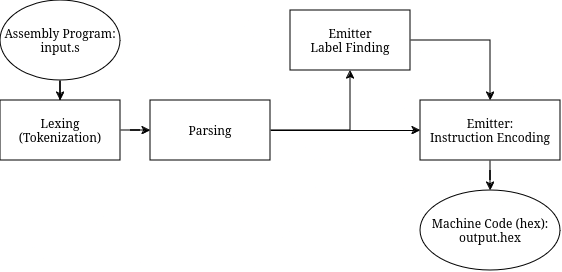
\includegraphics[width=0.8\linewidth]{Flowchart.png}

\subsection{Lexer / Tokenizer}

The assembler has a highly optimized lexer which scans the input 
program and generates {\em tokens}. A token is the smallest unit
of a program, such as an identifier, a numeric literal, or 
special characters like colons and commas.

$$
\underbrace{L1}_{ident}\ \underbrace{:}_{colon}\ \underbrace{lui}_{ident}\ \underbrace{x3}_{ident}\ \underbrace{,}_{comma}\ \underbrace{0{\times}1000}_{hexnum}
$$

The lexer assigns types to portions of the assembly program based
on their syntactic meaning. A \texttt{Token} is defined as follows:

\begin{verbatim}
typedef struct Token {
    TokenType type;
    Span span;	
} Token;
\end{verbatim}

\texttt{Span} is a struct that holds the start and end positions of a token:

\begin{verbatim}
typedef struct Span {
    size_t start, end;
} Span;
\end{verbatim}

The \texttt{TokenType} is an enum which denotes the token type
assigned to that portion of the source code.

\begin{verbatim}    
typedef enum TokenType {
    TOK_EOF, TOK_ERR,   // Tokens for end-of-file and syntax errors
    TOK_IDENT,
    TOK_DECNUM, TOK_BINNUM, TOK_HEXNUM, TOK_OCTNUM,
    TOK_COMMA, TOK_COLON, TOK_LPAREN, TOK_RPAREN,
} TokenType;
\end{verbatim}

The lexer itself requires a struct storing peroperties such As
the source string and the current position. 

\begin{verbatim}
typedef struct Lexer {
    char *src;
    size_t pos, line, lastline;
} Lexer;
\end{verbatim}

\texttt{line} and \texttt{lastline} hold the current line number,
and the position of the last newline character respectively. These
are used in error reporting.

The lexer API is very simple and has only two functions:

\begin{verbatim}
void lexer_init(Lexer* l, char *src);
Token lexer_next(Lexer *l);
\end{verbatim}

\texttt{lexer\_init} is used to initialize the lexer object.
\texttt{lexer\_next} returns the next token in the source code,
based on the current position of the lexer.

\subsection{Lookup Tables}

An assembler needs to maintain a list of instructions supported broadly
the ISA, the syntax of each instruction, and the operands it takes.

To do this, the assembler uses lookup tables, which map the name of
an insturction to attributes such as the instruction format, the operands
and \texttt{funct3} and \texttt{funct7} values.

For example, the lookup table for S-format instructions is defined as
follows:

\begin{verbatim}
SInsTableEntry s_ins_table[] = {
    {"sb", 0b0100011, 0x0},
    {"sh", 0b0100011, 0x1},
    {"sw", 0b0100011, 0x2},
    {"sd", 0b0100011, 0x3},
};
\end{verbatim}

where each entry is of the type:

\begin{verbatim}
typedef struct SInsTableEntry {
    char *key;
    int opcode, funct3;
} SInsTableEntry;    
\end{verbatim}

Similar tables are defined for instructions in other formats. These
lookup tables are used by the parser to identify an instruction's
format and syntax, and call the corresponding procedures.

One notable distinction is the existence of two tables for I-format
instructions:

\begin{verbatim}
IInsTableEntry i_ins_table[] = {
    {"addi", 0b0010011, 0x0},
    // ...
    {"srai", 0b0010011, 0x5},
};

IInsTableEntry i_ins_table_2[] = {
    {"lb", 0b0000011, 0x0},
    // ...
    {"jalr", 0b1100111, 0x0}
};
\end{verbatim}

This distinction is due to I-format instructions having two different syntaxes.
Arithmetic instructions are written as \texttt{addi rs, rs1, imm} while memory
based instructions are written as \texttt{ld rs2, imm(rs1)}.

Having a separate lookup table for each syntax simplifies the parsing of these
instructions.

The assembler also maintains a mapping of register names to register numbers:

\begin{verbatim}
RegTableEntry reg_table[] = {
    {"zero", 0},
    {"ra", 1},
    // ...
};
\end{verbatim}

Where each entry is of the form:

\begin{verbatim}
typedef struct RegTableEntry {
    char *key;
    int value;
} RegTableEntry;
\end{verbatim}

\subsection{Parser}

The parser works in tandem with the lexer to convert sequences of tokens
into semantic elements such as instructions and labels.

The parser works in tanden with the lexer. It requests tokens from the
lexer and emits a \texttt{ParseNode} object, defined as:

\begin{verbatim}    
typedef struct ParseNode {	
    NodeType type;
    union {
        Label l;
        RIns r;
        IIns i;
        SIns s;
        BIns b;
        UIns u;
        JIns j;
    } data;
    int line;
} ParseNode;
\end{verbatim}

The struct is essentially a tagged union, containing data corresponding either to a label or 
to one of the six instruction types. The line number of the element is also stored to
facilitate error reporting in the emitter.

The enum \texttt{NodeType} just indicates the type of the node (i.e which field of the union to
access), and is defined as:

\begin{verbatim}
typedef enum NodeType {
    LABEL, R_INS, I_INS, S_INS, B_INS, U_INS, J_INS
} NodeType;
\end{verbatim}

The structs for instructions are pretty similar. They hold
data about the instruction's fields (opcode, funct3, funct7),
and the operands (registers and immediate). For example,
\texttt{RIns} is defined as follows:

\begin{verbatim}
typedef struct RIns {
    RInsTableEntry *entry;
    int rd, rs1, rs2;
} RIns;
\end{verbatim}

\texttt{entry} is an element of the lookup table for R-instructions,
detailed in the previous section.

The parser itself is defined as:

\begin{verbatim}
typedef struct Parser {
    Token current;
    Lexer *lexer;
    char *src;
} Parser;
\end{verbatim}

The section on bottom-up parsing gives an outline of the parser.
Two public functions are defined:
\begin{verbatim}
// Initializes the parser
void parser_init(Parser *p, Lexer *l);

// Parses and returns a single semantic element
ParseNode parser_next(Parser *p, ParseErr *err);
\end{verbatim}

\texttt{parser\_next} first compares the current token
with various instruction names. By doing this, it
identifies the instruction format, and calls the function
responsible for parsing that instruction.

If the token does not match any of the instrucion, then
it checks if the token corresponds to a label definitions
(identifier followed by colon). If that too does not match,
then it raises an error.

\subsubsection{Parsing Immediates}

Instructions often take an immediate as an operand. In
the case of I-, S- and U-format instructions, these
are often numeric literals, but in the case of B- and
J- format instructions, both numeric literals and labels
are used as immediates.

Hence, it is necessary to account for both cases - labels
and numeric literals. This is done using a struct called 
\texttt{NumOrLabel}:

\begin{verbatim}
typedef struct NumOrLabel {
    int is_label;
    union {
        int n;
        Label l;
    } data;
} NumOrLabel;    
\end{verbatim}

This is a tagged union which can hold either a label or a numeric literal.

\subsection{Emitter}

The emitter takes the parse tree as input and emits
machine code. This is done in two steps. First it
finds and enumerates all the labels in the parse
tree. Then it converts instructions to the machine
code equivalent.

The emitter also has an error handling system which
is very similar to the parser. The \texttt{EmitErr}
struct is used for this purpose.

\begin{verbatim}
typedef struct EmitErr {
    int is_err;
    char *msg;
    int line;
} EmitErr;
\end{verbatim}

This struct is similar to \texttt{ParseErr} except that
the column span for the error are not stored.

Since RISC-V immediates are encoded into the instruction,
they have to fit in a certain number of bits. The emitter
performs bounds checking for these immediate values.

In addition to this, the emitter also handles cases where
an undefined label is used in the program, or a label
is defined multiple times.

\section{Features}
The assembler satisfies the following requirements:

\begin{itemize}
    \item Supports all RV64I Base Integer Instructions
    \item Supports both standard RISC-V register names and calling convention aliases
    \item Supports decimal, hexadecimal, binary and octal numeric literals.
    \item Reports errors in the program along with their line numbers.
    \item Supports comments starting with the \texttt{;} character.
    \item Flexible parsing allowing for extra whitespace between tokens.
\end{itemize}
The assembler handles the following kinds of errors:

\begin{itemize}
    \item Syntax errors
    \item Invalid instruction and register names
    \item References to undefined labels
    \item Redefinition of a label
    \item Labels without instructions (e.g. at end of file)
    \item Immediates not fitting in instruction field
    \item Branch and jump immediates being odd numbers
\end{itemize}

\section{Testing}

The project includes a few testcases in the \texttt{test/} directory.
A bash script, \texttt{test.sh}, is used to run all the tests.
Each test includes an assembly program \texttt{input.s} and the
expected output \texttt{expected.hex}.

The testcases include examples from the problem statement, as well as
some miscellaneous programs.

\section{Future Scope}

The assembler can be extended further in future to make it a more 
practical tool. Some possible features include
\begin{itemize}
    \item Ability to report multiple errors in the same program.
    \item Support for RISC-V pseudo-instructions.
    \item Support for \texttt{.data} section.
\end{itemize}

\section{Project File Structure}

\begin{verbatim}
    .
    |-- Makefile
    |-- report
    |   |-- (...)
    |   |-- main.tex    (Source file for the report)
    |-- src
    |   |-- emitter.c   (Source code for emitter)
    |   |-- emitter.h
    |   |-- lexer.c     (Source code for lexer)
    |   |-- lexer.h
    |   |-- main.c      (Driver code for the assembler)
    |   |-- parser.c    (Source code for the parser)
    |   |-- parser.h
    |   |-- tables.c    (Instruction and register tables)
    |   `-- tables.h
    |-- test            (Test cases)
    `-- test.sh         (Script for running tests)
\end{verbatim}

\end{document}